\documentclass{beamer}
\usetheme{metropolis} 
\usepackage{listings}
\usepackage{xcolor}
\definecolor{myBlue}{RGB}{0, 0, 180}
\definecolor{myGreen}{RGB}{34, 139, 34}
\definecolor{myRed}{RGB}{180, 0, 0}
\definecolor{myGray}{RGB}{96, 96, 96}
\lstset{ 
    language=Python,
    basicstyle=\ttfamily\tiny,
    keywordstyle=\color{myBlue},
    commentstyle=\color{myGreen},
    stringstyle=\color{myRed},
    showstringspaces=false,
    numberstyle=\tiny\color{myGray},
    stepnumber=1,
    numbersep=5pt,
    frame=single,
    breaklines=true,
    breakatwhitespace=true,
    tabsize=4,
    captionpos=b
}
\title{Artificial Intelligence, Algorithmic Pricing, and Collusion}
\subtitle{Emilio Calvano, Giacomo Calzolari, Vincenzo Denicol\`{o}, and Sergio Pastorello}
\date{\today}
\author{Gabe Sekeres and Finn Ye}
\institute{Cornell University}
\begin{document}


\begin{frame}
	\titlepage
\end{frame}


\section{Background}

\begin{frame}\frametitle{Motivation}
	\begin{itemize}
		\item Algorithms becoming increasingly prevalent in practice
		\begin{itemize}
			\item German gasoline markets (Assad et al. 2024)
			\item Smartphone price discrimination (Kehoe et al. 2020)
		\end{itemize}
		\item Regulatory questions: \begin{itemize} \item How do algorithms get to collusive prices? \item Can they do so in the absence of active principals? \item Is algorithmic collusion visibly different than tacit collusion? \end{itemize}
		\item Massive lack of theoretical guarantees for this (see Banchio and Mantegazza (2023); Possnig (2024); Lamba and Zhuk (2025))
	\end{itemize}	
\end{frame}

\begin{frame}\frametitle{Q-Learning Algorithms}
	\begin{itemize}
		\item We're familiar with Q-learners 
		\item Specifically, they learn \emph{slowly}. This example has a massive state space and is trying to learn the opponent's policy as part of the state
		\item Our biggest criticisms are related to this. Specifically: \begin{itemize} \item What is the loss in the learning phase? \item How sensitive are these results to the initialization of the Q-matrix?\end{itemize}
	\end{itemize}
\end{frame}

\section{Model}

\begin{frame}\frametitle{Environment}
	Canonical oligopoly pricing game, with $n$ firms / products and an outside good, where in each period $t$ the demand for good $i$ is \[q_{i,t} = \frac{e^{\frac{a_i-p_{i,t}}{\mu}}}{\sum_{j=1}^n e^{\frac{a_j - p_{j,t}}{\mu}} + e^{\frac{a_0}{\mu}}}\]where $a_i$ is an index of quality, $\mu$ is in index of differentiation, and $a_0$ is an outside good. Firms choose $p_{i,t}$, and we have exogenous marginal costs $c_i$. The stage problem is:\[\max_{p_{i,t}} q_{i,t}(p_{i,t}) \cdot p_{i,t} - q_{i,t}(p_{i,t}) \cdot c_{i,t}\]This is quasiconcave but does not in general have a nice closed form solution.
\end{frame}
\begin{frame}\frametitle{Simplified Stage Environment}
	Assume $n=2$, $c_i = 1$, $a_i = 2$, $a_0=0$, and $\mu = \frac{1}{4}$. Then the stage game reduces to\[\max_{p_i} \frac{(p_i - 1)e^{8 - 4p_{i}}}{e^{8 - 4p_{i}} + e^{8 - 4p_{j}} + 1}\]This is strictly concave, and we have that it admits Nash prices\[p^N_i = p^N_j \approx 1.473\]and monopoly prices are obtained from setting $n=1$, where we attain \[p^M = \frac{5}{4} - \frac{1}{4}W_n(2e^{3}) \approx 1.925\]
\end{frame}
\begin{frame}\frametitle{Simplified Stage Environment}
	We basically have an extension of a Prisoner's Dilemma:
	\[
	\begin{array}{c|cc}
		& N & M \\\hline N & (0.22,0.22) & (0.37,0.12) \\ M &(0.12,0.37) & (0.34,0.34)
	\end{array}	\]
	Since all of the involved functions are continuous and concave, this extends fairly nicely. 
	
	So we're making our Q-learners play a repeated Prisoner's Dilemma, and the strategies they learn \emph{should} be similar to canonical repeated PD strategies. 
\end{frame}

\begin{frame}\frametitle{Folk Theorem}
\begin{center}
	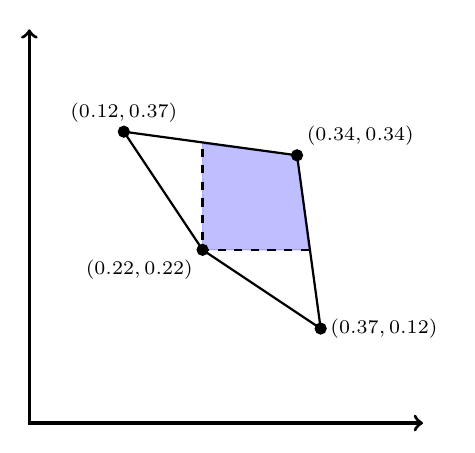
\begin{tikzpicture}[scale=1]
		\filldraw[blue,nearly transparent] (3.4,3.4)--(3.55,2.2)--(2.2,2.2)--(2.2,3.55)--(3.4,3.4);
		\draw[very thick, <->] (0,5)--(0,0)--(5,0);
		\draw[thick] (2.2,2.2)--(1.2,3.7)--(3.4,3.4)--(3.7,1.2)--(2.2,2.2);
		\filldraw (2.2,2.2) circle(2pt);
		\filldraw (1.2,3.7) circle(2pt);
		\filldraw (3.7,1.2) circle(2pt);
		\filldraw (3.4,3.4) circle(2pt);
		\draw[dashed,thick] (3.55,2.2)--(2.2,2.2)--(2.2,3.55);
		\node[below left] at (2.2,2.2) {\scriptsize$(0.22,0.22)$};
		\node[above right] at (3.4,3.4) {\scriptsize$(0.34,0.34)$};
		\node[right] at (3.7,1.2) {\scriptsize$(0.37,0.12)$};
		\node[above] at (1.2,3.7) {\scriptsize$(0.12,0.37)$};
	\end{tikzpicture}
\end{center}
\end{frame}

\begin{frame}\frametitle{Continuous Stage Payoffs}
	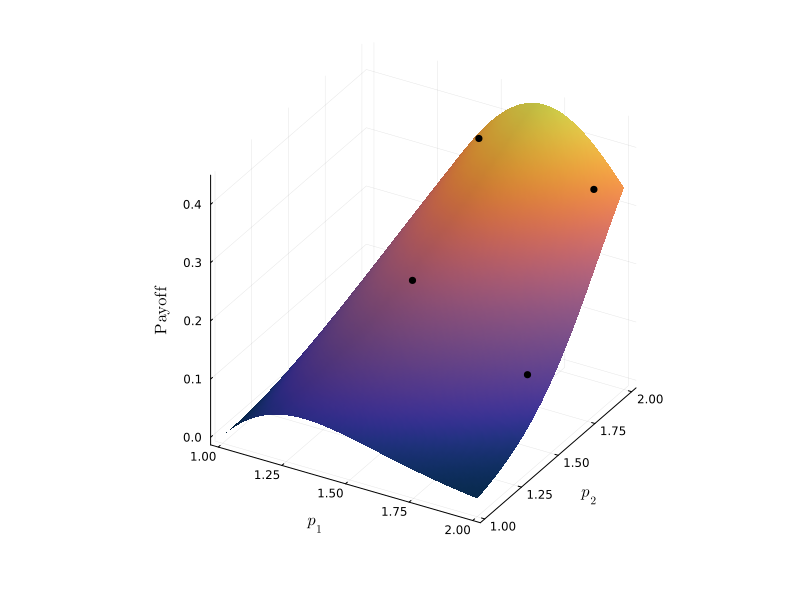
\includegraphics[width=10cm]{cont_plot.png}
\end{frame}

\begin{frame}\frametitle{A Question}
	Why use this sigmoid demand function instead of exogenously imposing a reasonable range for prices and using \emph{e.g.} linear demand?
	
	We don't understand what the gain from this functional form is, and the fact that it doesn't in general have closed-form solutions is an annoyance.
\end{frame}

\section{Learning Theory}

\begin{frame}\frametitle{Learning in Repeated Games}
	Essentially, take the opponent's previous actions to be the state, along with whatever game parameters you need. Two issues:
	\begin{enumerate}
		\item The state space is increasing as the game continues. \\ Solution: Bounded memory. 
		\item The optimization problem is non-stationary if the opponent(s) change strategy over time. \\ No official solutions here, this is why we don't have theoretical guarantees\footnote{I'm fairly sure there should be something here. At least in probability. I'm confused why nobody has proved that yet - Gabe}
	\end{enumerate}
\end{frame}

\begin{frame}\frametitle{Learning in Repeated Games}
	The Q-learners solve \[Q(s,a) = \mathbb{E}(\pi \mid s,a) + \delta \mathbb{E}\left[ \max_{a'\in A} Q(s',a') \mid s,a\right]\] where $a \in A$ is the action (from the rules of the game), $s \in S$ is the state (defined as all player actions in the last $k$ periods, where $k$ is the memory). Once we discretize, $Q \in \mathbb{R}^{|A| \times |S|} = \mathbb{R}^{|A| \times |A|^{nk}}$
	
	For simplicity, $k=1$. Results robust to higher $k$.
\end{frame}

\begin{frame}\frametitle{Parameterization}
	Work in the simplified game as above, with $\delta = 0.95$ and $|A| = m = 15$. Discretize the price grid over \[\left[p^N - 0.1(p^M - p^N), p^M + 0.1(p^M - p^N)\right]\] Set the initial matrix to the discounted payoff if the other player randomized over all actions: \[Q_{i,0}(s,a_i) = \frac{\sum_{a_{-i} \in A^{n-1}}\pi_i(a_i,a_{-i})}{(1-\delta) |A|^{n-1}}\]Draw the initial state $s_0$ randomly as well.
\end{frame}

\begin{frame}\frametitle{Continuous Stage Payoffs}
\centering
	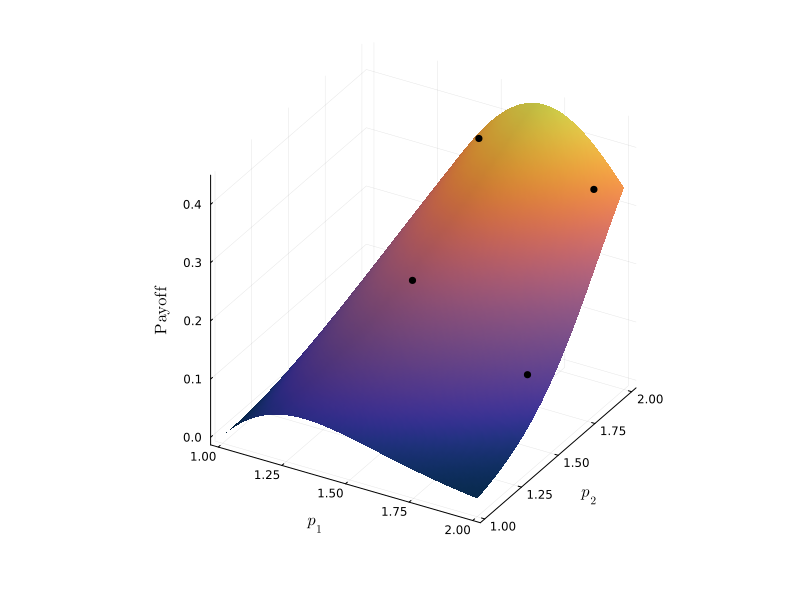
\includegraphics[width=10cm]{cont_plot.png}
\end{frame}
\begin{frame}\frametitle{Discretized Stage Payoffs}
\centering
	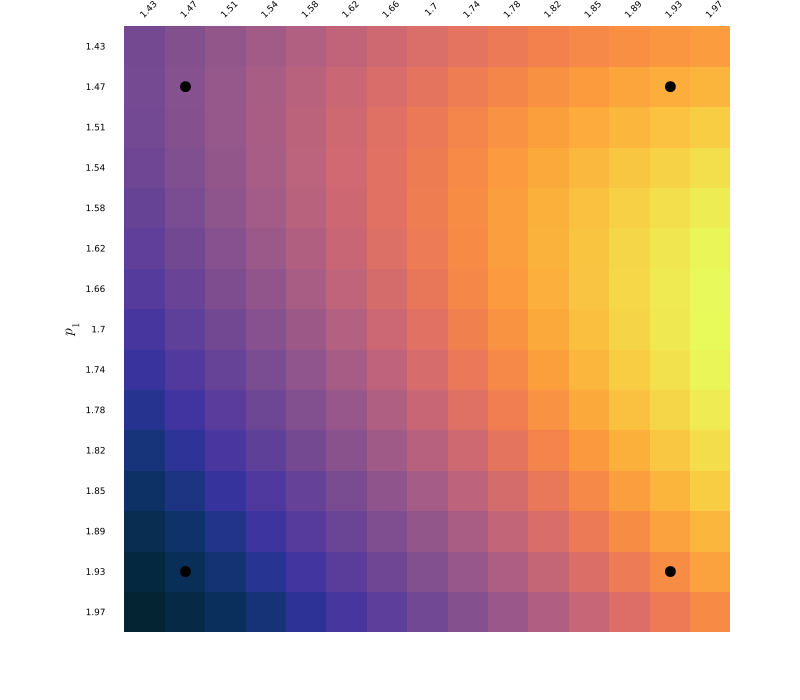
\includegraphics[width=8cm]{heatmap_plot.png}
\end{frame}

\begin{frame}\frametitle{Parameterization}
	We will use $\varepsilon$-greedy learners, with $\varepsilon_t = \exp(-\beta t)$. The learning parameter $\alpha$ will be tested over a grid of 100 points in $[0.025, 0.25]$, and several different values of $\beta$ are also tested. 
	
	They define $\nu$ to be the number of times a certain cell is visited in expectation under a certain $\beta$. For our purposes, $\beta$ will be tested over a grid of 100 points in $(0,2 \cdot 10^{-5})$. 
	
	Recall from earlier:\[Q(s,a) \leftarrow Q(s,a) + \alpha \left[ \pi(s',a') + \delta \max_{a'\in A} Q(s',a') - Q(s,a)\right]\]
\end{frame}

\begin{frame}\frametitle{Learning Visualization}
	\centering
	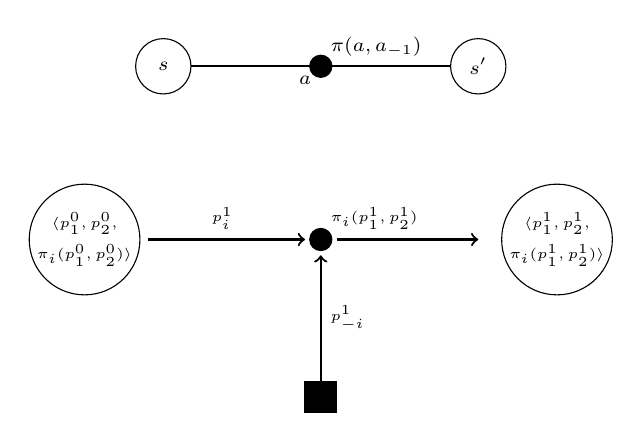
\begin{tikzpicture}[scale=2]
		\draw[thick] (0,0)--(2,0);
		\filldraw[color=black, fill=white] (0,0) circle(5pt);
		\node at (0,0) {\scriptsize$s$};
		\filldraw (1,0) circle(2pt);
		\filldraw[color=black, fill=white] (2,0) circle(5pt);
		\node at (2,0) {\scriptsize$s'$};
		\node[above right] at (1,0) {\scriptsize$\pi(a,a_{-1})$};
		\node[below left] at (1,0) {\scriptsize$a$};
		\filldraw[color=black, fill=white] (-0.5,-1.1) circle(10pt);
		\node at (-0.5,-1) {\tiny$\langle p_1^{0},p_{2}^{0},$};
		\node at (-0.5,-1.2) {\tiny$\pi_i(p_1^{0},p_{2}^{0}) \rangle$};
		\draw[thick,->] (-0.1,-1.1) -- (.9,-1.1);
		\node[above] at (.375,-1.1) {\tiny$p_i^1$};
		\draw[thick,->] (1,-2) -- (1,-1.2);
		\filldraw (1,-1.1) circle(2pt);
		\node[right] at (1,-1.6) {\tiny$p_{-i}^1$};
		\node[above right] at (1,-1.1) {\tiny$\pi_i(p_1^1,p_2^1)$};
		\filldraw (0.9,-2)--(1.1,-2)--(1.1,-2.2)--(0.9,-2.2)--(0.9,-2);
		\draw[thick,->] (1.1,-1.1)--(2,-1.1);
		\filldraw[color=black, fill=white] (2.5,-1.1) circle(10pt);
		\node at (2.5,-1) {\tiny$\langle p_1^{1},p_{2}^{1},$};
		\node at (2.5,-1.2) {\tiny$\pi_i(p_1^{1},p_{2}^{1}) \rangle$};
	\end{tikzpicture}
\end{frame}

\begin{frame}\frametitle{Remark}
	In the paper, they say that their results are robust to many specifications of $Q_0$, the initial matrix.
	
	We did not see that.
	
	We saw results that changed a lot depending on $Q_0$. 
	
	Specifically, their results were \emph{only} replicated by their specific choice of $Q_0$. If you initial $Q_0 = 0$ for all values, they converge to the static Nash payoffs necessarily.
\end{frame}

\begin{frame}\frametitle{Remark}
	Prior to this, we've generally dealt with RL algorithms that are trying to learn \alert{payoffs} in a static or stochastic game. These algorithms are (theoretically) learning \alert{strategies} for the infinitely repeated game. 
	
	Thinking about the bounded memory, that's no longer such an innocuous assumption. For example: these algorithms will be able to learn tit-for-tat or Grim Trigger, but not trigger strategies with $n$ periods of punishment for $n > k$.
\end{frame}


\section{Code}


\section{Results}






























	
\end{document}
